% SNU Central: IEEE conference paper (IEEEtran). Compile with pdfLaTeX on Overleaf (no BibTeX step needed).
\documentclass[conference]{IEEEtran}
\IEEEoverridecommandlockouts

\usepackage[T1]{fontenc}
\usepackage{cite}
\usepackage{amsmath,amssymb,amsfonts}
\usepackage{graphicx}
\usepackage{booktabs}
\usepackage{multirow}
\usepackage{array}
\usepackage{tabularx}
\usepackage{xcolor}
\usepackage{url}
\usepackage{tikz}
\usetikzlibrary{arrows.meta,positioning,shapes.geometric,fit,backgrounds,calc}
\usepackage[hidelinks]{hyperref}

\definecolor{ieeeblue}{HTML}{2A78D6}
\definecolor{ieeeorange}{HTML}{EB6834}
\definecolor{boxgray}{HTML}{F2F2F0}
\newcommand{\code}[1]{\texttt{#1}}
\newcolumntype{L}[1]{>{\raggedright\arraybackslash}p{#1}}
\newcolumntype{Y}{>{\raggedright\arraybackslash}X}
\renewcommand{\arraystretch}{1.12}

\begin{document}

\title{SNU Central: A Citation-Grounded Retrieval-Augmented Question Answering System for University Policy Documents}

\author{
\IEEEauthorblockN{Poorab Mishra (2310110721), Vishnu Chundu (2310110358),\\
Shreyas Achal (2310110289), Mitaksh Goswami (2410110875)}
\IEEEauthorblockA{\textit{Department of Computer Science and Engineering}\\
\textit{Shiv Nadar Institution of Eminence}\\
Delhi-NCR, India\\
\href{https://github.com/MajinVegetaaa/SNUCentral}{\texttt{github.com/MajinVegetaaa/SNUCentral}}}
}

\maketitle

% ---------------------------------------------------------------------------------------------------
\begin{abstract}
University students often struggle to find answers to policy questions because the relevant rules are scattered across long PDF documents on several platforms and are written in formal language. We present SNU Central, a retrieval-augmented question-answering system that answers questions about Shiv Nadar University's policies using only official documents, and links every claim to the document, page, section and paragraph it came from. The system indexes 39 public policy documents (660 pages, 2{,}801 passages) with an inverted index, TF-IDF and BM25 ranking, synonym expansion and spelling correction, all implemented from scratch. An open-weight language model, \code{gpt-oss-120b}, phrases answers solely from the retrieved passages; it may cite only passage numbers, which the application validates and converts into citations from metadata. A length-normalised BM25 confidence gate declines clearly off-topic questions before the model is called. On a hand-labelled test set of 25 questions, BM25 outperformed TF-IDF (MRR 0.792 vs.\ 0.581; F1@5 0.609 vs.\ 0.453). The system declined all five unanswerable questions without refusing any answerable one, and 95\% of its answers were factually correct. At the statement level, 94\% of answer statements were supported by a cited passage, and every cited statement was supported by its citation, whereas an audit of commercial generative search engines, in a broader open-web setting, found 51.5\% of sentences supported. Spelling correction recovered the full retrieval loss caused by typos. The system runs on an 8\,GB laptop at no cost and answers in under two seconds.
\end{abstract}

\begin{IEEEkeywords}
information retrieval, BM25, TF-IDF, inverted index, retrieval-augmented generation, question answering, source attribution, citation verification, hallucination, abstention, spelling correction
\end{IEEEkeywords}

% ---------------------------------------------------------------------------------------------------
\section{Introduction}

\subsection{Background}
Universities govern student life through a large body of institutional documents: academic regulations, attendance and grading policies, examination manuals, codes of conduct, fee policies, hostel rules and official circulars. At Shiv Nadar University (SNU) these documents are spread across the university website, the SNU Links policy portal, handbooks and individual PDF circulars, and many are long; the fee policy alone runs to 198 pages. The information students need is usually present. The difficulty lies in \emph{locating, accessing and understanding} it: a student must first guess which document holds the answer, then search a long PDF for the right clause, and then interpret formal policy language.

\subsection{Importance of the Problem}
The project brief identifies five problems with the current process: (1)~\emph{fragmented information} across websites, portals and departments; (2)~\emph{difficult navigation} of lengthy PDFs; (3)~\emph{keyword-dependent search} that misses questions phrased differently from the policy (``drop a course'' versus ``withdrawal''); (4)~\emph{hard-to-understand} formal language; and (5)~\emph{no direct references} to the provision that supports an answer. Policy questions have consequences: a misread attendance rule can bar a student from an examination. An assistant for this setting must therefore meet a stricter standard than a general chatbot: every answer must be traceable to the official text, and the system must say so when the documents do not contain an answer.

\subsection{Motivation}
Large language models (LLMs) can turn formal policy text into clear answers, but on their own they know nothing about a particular university's rules and are prone to \emph{hallucination}, fluent statements that no source supports~\cite{ji2023hallucination}. Retrieval-augmented generation (RAG) conditions the model on retrieved passages~\cite{lewis2020rag}, but a RAG system is only as reliable as its retrieval step, and its answers are only verifiable if their citations can be checked~\cite{gao2023alce}. Following the brief's principles of \emph{retrieval before generation}, \emph{source transparency} and \emph{accuracy over assumptions}, we build the retrieval core from classical, inspectable techniques, an inverted index with TF-IDF and BM25 ranking~\cite{salton1988term,robertson2009bm25}, and use the LLM only as a thin language layer that rephrases what retrieval has found.

\subsection{Contributions}
\begin{enumerate}
\item \textbf{A citable corpus} of 39 official SNU documents from four public sources, split into 2{,}801 paragraph-level passages that keep their document, page, section, paragraph and date. Dates are read from the documents themselves, which dates 34 of 39 documents without guessing.
\item \textbf{A from-scratch IR engine} (inverted index, TF-IDF with cosine similarity, Okapi BM25) with a measured comparison: BM25 reaches an MRR of 0.792 against 0.581.
\item \textbf{Citation-grounded generation}: the LLM writes only passage markers such as \code{[3]}; the application builds citations from metadata and rejects markers that point to no retrieved passage.
\item \textbf{Two-layer abstention}: a BM25 confidence gate before any LLM call, then a prompt-level refusal. All five off-topic test questions are declined with no false refusals.
\item \textbf{Spelling correction} with a character $k$-gram index and Damerau--Levenshtein distance, restoring 20 of 20 typo-corrupted queries.
\item \textbf{A two-level evaluation} of retrieval (precision, recall, F1, MRR) and answers, including \emph{statement-level groundedness}: 85 of 90 statements (94\%) are supported by a cited passage.
\item \textbf{A working, zero-cost system} that runs on an 8\,GB laptop, answers in under two seconds, and still shows cited passages when the LLM is unavailable.
\end{enumerate}

Section~\ref{sec:related} reviews related work, Section~\ref{sec:objective} states the objectives, Section~\ref{sec:model} presents the system, Section~\ref{sec:method} the algorithms, Section~\ref{sec:results} the experiments, and Section~\ref{sec:conclusion} concludes.

% ---------------------------------------------------------------------------------------------------
\section{Related Work}\label{sec:related}

\subsection{Term Weighting and Probabilistic Ranking}
Salton and Buckley~\cite{salton1988term} showed that single terms with suitable weights, combining term frequency, inverse document frequency and length normalisation, retrieve better than more elaborate representations; their tf$\cdot$idf scheme with cosine normalisation is our baseline. Robertson and Zaragoza~\cite{robertson2009bm25} derive BM25 from the probabilistic relevance framework; it adds term-frequency saturation ($k_1$) and document-length normalisation ($b$). Manning et al.~\cite{manning2008ir} give the textbook treatment of the inverted index, the evaluation measures we use, and isolated-term spelling correction with $k$-gram indexes and edit distance. Damerau~\cite{damerau1964} introduced the edit operation that counts a swap of adjacent letters as one error, which our speller uses.

\subsection{Dense Retrieval and the Strength of BM25}
Dense Passage Retrieval~\cite{karpukhin2020dpr} encodes questions and passages with BERT and beats a BM25 baseline by 9--19 points in top-20 accuracy when trained on in-domain QA data. The BEIR benchmark~\cite{thakur2021beir} (18 datasets, 10 systems), however, showed that in zero-shot use on new domains BM25 remains a robust baseline and dense retrievers often generalise poorly. University policy text is a new domain with no training data, and our system must run on a laptop at no cost, so BM25 is the safest and most practical first choice.

\subsection{Retrieval-Augmented Generation}
Lewis et al.~\cite{lewis2020rag} introduced RAG, which conditions a sequence-to-sequence generator on passages selected by a neural retriever, producing more specific and factual answers than a generator alone. We keep the retrieve-then-generate idea but use a classical retriever and an off-the-shelf open-weight LLM that is only prompted, never trained, so the ranking step stays transparent and testable on its own.

\subsection{Hallucination, Attribution and Citations}
Ji et al.~\cite{ji2023hallucination} survey hallucination across generation tasks and identify retrieval grounding as a main mitigation. Rashkin et al.~\cite{rashkin2023ais} define \emph{Attributable to Identified Sources} (AIS): a statement is acceptable only if a reader could confirm it from an identified source, which motivates our statement-level grading. Gao et al.~\cite{gao2023alce} built the ALCE benchmark for LLM answers with citations and found that even the best models lacked complete citation support for about half of their long-form answers. Liu et al.~\cite{liu2023verifiability} audited four commercial generative search engines and found only 51.5\% of sentences fully supported by their citations and only 74.5\% of citations supporting their sentence.

\subsection{Evaluating RAG and University Assistants}
RAGAS~\cite{es2024ragas} scores RAG pipelines without references by using an LLM as the judge; we instead report standard IR metrics on hand-labelled judgments, manual grading and deterministic checks. BarkPlug v.2~\cite{neupane2024barkplug} is a RAG chatbot for Mississippi State University's campus resources that reports a mean RAGAS score of 0.96 and a user survey; its summary does not report run-time citation verification or abstention before the LLM is called, the two properties we focus on.

\subsection{Novelty}
Table~\ref{tab:related} compares SNU Central with the closest work. Our contribution is a \emph{transparent, verifiable pipeline} for a high-stakes domain: (1)~the application, not the model, produces each citation, so the model cannot invent a document or page; (2)~abstention happens before generation when retrieval finds nothing relevant; (3)~the retriever is classical, inspectable and evaluated on its own; and (4)~groundedness is measured per statement.

\begin{table*}[t]
\caption{Comparison of SNU Central with Related Systems}
\label{tab:related}
\centering
\footnotesize
\begin{tabularx}{\textwidth}{@{}L{3.0cm}YYYYY@{}}
\toprule
 & \textbf{RAG}~\cite{lewis2020rag} & \textbf{ALCE}~\cite{gao2023alce} & \textbf{Generative search}~\cite{liu2023verifiability} & \textbf{BarkPlug v.2}~\cite{neupane2024barkplug} & \textbf{SNU Central (ours)} \\
\midrule
Retriever & Dense (DPR), trained & Dense / web search & Web search & LLM-based RAG stack & Own BM25 / TF-IDF over an inverted index \\
Citations in answer & No & Yes, generated by LLM & Yes & Not reported & LLM writes \code{[n]}; app builds citation from metadata \\
Citations verified against retrieved passages & -- & Measured offline & Audited offline & -- & Every answer, at run time; invalid markers removed \\
Abstains before calling the LLM & No & No & No & No & Yes, BM25 confidence gate \\
Link to exact source page & No & No & URL only & Not reported & Document, page, section, paragraph, date \\
Retrieval evaluation & QA accuracy & -- & -- & RAGAS & P@5, R@5, F1@5, MRR on 92 judgments \\
Answer evaluation & Exact match & Citation recall/precision & Human audit & RAGAS, SUS survey & Manual correctness, completeness, statement-level support \\
Cost / hardware & GPU training & Commercial LLMs & Commercial services & Hosted LLMs & \$0, 8\,GB laptop, free-tier open-weight LLM \\
\bottomrule
\end{tabularx}
\end{table*}

% ---------------------------------------------------------------------------------------------------
\section{Objective}\label{sec:objective}

The aim of SNU Central is to provide a single platform through which students can ask about university policies in their own words and receive clear answers that are supported by, and linked to, the original documents. Following the project brief, information should be \emph{accessible} (one interface for all offices), \emph{searchable} (no need to know the document or exact wording), \emph{understandable} (plain answers that keep every condition, number and deadline), \emph{verifiable} (document, page, section and paragraph, with a link to the page) and \emph{reliable} (no unsupported answers).

The specific objectives are to: \textbf{O1}~build a corpus of official documents with full provenance and citable passages; \textbf{O2}~implement tokenisation, stemming, an inverted index, TF-IDF and BM25 ourselves; \textbf{O3}~compare the two rankers on labelled questions; \textbf{O4}~generate answers only from retrieved passages, with citations produced and checked by the application; \textbf{O5}~decline questions the documents cannot answer, preferably before any LLM call; \textbf{O6}~make search robust through synonyms and spelling correction; \textbf{O7}~evaluate answers separately from retrieval; and \textbf{O8}~run on an 8\,GB laptop at no cost and degrade gracefully without the LLM. Table~\ref{tab:targets} lists the targets fixed in the requirements before evaluation.

\begin{table}[t]
\caption{Targets Fixed Before the Evaluation}
\label{tab:targets}
\centering
\footnotesize
\begin{tabular}{@{}lr@{}}
\toprule
\textbf{Criterion} & \textbf{Target} \\
\midrule
MRR of the better ranker & $\geq 0.70$ \\
Precision@5 of the better ranker & $\geq 0.60$ \\
Answer statements supported by a cited passage & $\geq 90\%$ \\
Correct abstention on unanswerable questions & $\geq 80\%$ \\
Citations to the correct document, page, paragraph & $100\%$ \\
Retrieval time / complete answer & $<500$\,ms / $\approx 5$\,s \\
\bottomrule
\end{tabular}
\end{table}

The evaluation answers four research questions. \textbf{RQ1}: does BM25 retrieve more relevant policy passages than TF-IDF with cosine similarity? \textbf{RQ2}: can a classical retriever with a confidence threshold separate answerable from unanswerable questions before calling an LLM? \textbf{RQ3}: when the LLM is restricted to numbered passages and its citations are checked, what share of its statements are supported? \textbf{RQ4}: how much retrieval quality do typos cost, and how much does correction recover? Scanned documents, login-only documents, dense retrieval, follow-up questions and personal eligibility decisions are out of scope.

% ---------------------------------------------------------------------------------------------------
\section{Proposed Model}\label{sec:model}

SNU Central has two parts (Fig.~\ref{fig:pipeline}): an \emph{offline indexing pipeline} that turns official PDFs into an inverted index of citable passages, and an \emph{online answering pipeline} that retrieves passages, decides whether they are good enough to answer from, and only then asks an LLM for an answer whose citations the application checks. The IR engine works on its own; the LLM is a replaceable last step.

\begin{figure*}[t]
\centering
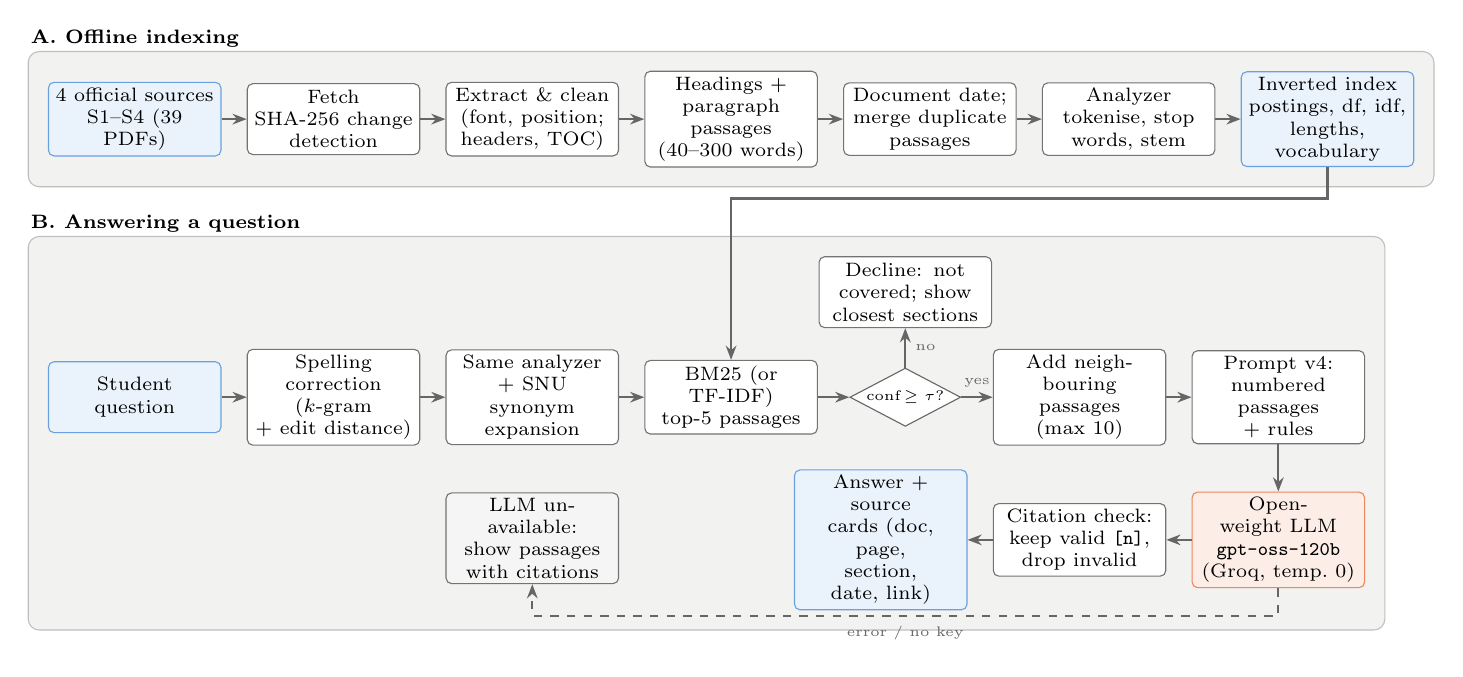
\begin{tikzpicture}[
  font=\scriptsize,
  node distance=4mm and 3.2mm,
  box/.style={draw=black!55, rounded corners=2pt, fill=white, align=center, minimum height=9mm, text width=2.05cm, inner sep=2pt},
  data/.style={box, fill=ieeeblue!10, draw=ieeeblue!70},
  llm/.style={box, fill=ieeeorange!12, draw=ieeeorange!80},
  decision/.style={diamond, aspect=1.9, draw=black!60, fill=white, align=center, inner sep=0.5pt, font=\tiny},
  arr/.style={-{Stealth[length=1.8mm]}, thick, black!60},
  lane/.style={draw=black!25, fill=boxgray, rounded corners=4pt, inner sep=2.5mm}
]
% ---- offline lane
\node[data] (src) {4 official sources\\S1--S4 (39 PDFs)};
\node[box, right=of src] (fetch) {Fetch\\SHA-256 change\\detection};
\node[box, right=of fetch] (ext) {Extract \& clean\\(font, position;\\headers, TOC)};
\node[box, right=of ext] (chunk) {Headings +\\paragraph passages\\(40--300 words)};
\node[box, right=of chunk] (date) {Document date;\\merge duplicate\\passages};
\node[box, right=of date] (ana1) {Analyzer\\tokenise, stop\\words, stem};
\node[data, right=of ana1] (idx) {Inverted index\\postings, df, idf,\\lengths, vocabulary};
\draw[arr] (src) -- (fetch); \draw[arr] (fetch) -- (ext); \draw[arr] (ext) -- (chunk);
\draw[arr] (chunk) -- (date); \draw[arr] (date) -- (ana1); \draw[arr] (ana1) -- (idx);

% ---- online lane, row 1
\node[data, below=26mm of src] (q) {Student\\question};
\node[box, right=of q] (spell) {Spelling\\correction ($k$-gram\\+ edit distance)};
\node[box, right=of spell] (ana2) {Same analyzer\\+ SNU synonym\\expansion};
\node[box, right=of ana2] (rank) {BM25 (or TF-IDF)\\top-5 passages};
\node[decision, right=4mm of rank] (gate) {conf\,$\geq\tau$?};
\node[box, right=4mm of gate] (ctx) {Add neighbouring\\passages\\(max 10)};
\node[box, right=of ctx] (prm) {Prompt v4:\\numbered passages\\+ rules};
% ---- online lane, row 2
\node[llm, below=6mm of prm] (llm) {Open-weight LLM\\\code{gpt-oss-120b}\\(Groq, temp.\ 0)};
\node[box, left=of llm] (val) {Citation check:\\keep valid \code{[n]},\\drop invalid};
\node[data, left=of val] (out) {Answer + source\\cards (doc, page,\\section, date, link)};
\node[box, above=5mm of gate] (abs) {Decline: not\\covered; show\\closest sections};
\node[box, below=6mm of ana2, fill=black!4] (fb) {LLM unavailable:\\show passages\\with citations};

\draw[arr] (q) -- (spell); \draw[arr] (spell) -- (ana2); \draw[arr] (ana2) -- (rank);
\draw[arr] (rank) -- (gate); \draw[arr] (gate) -- node[above, font=\tiny]{yes} (ctx);
\draw[arr] (ctx) -- (prm); \draw[arr] (prm) -- (llm);
\draw[arr] (llm) -- (val); \draw[arr] (val) -- (out);
\draw[arr] (gate.north) -- node[right, font=\tiny]{no} (abs.south);
\draw[arr, dashed] (llm.south) -- ++(0,-3.5mm) -| node[pos=0.25, below, font=\tiny]{error / no key} (fb.south);
\draw[arr] (idx.south) -- ++(0,-4mm) -| (rank.north);

% ---- lanes
\begin{scope}[on background layer]
\node[lane, fit=(src)(idx)] (offl) {};
\node[lane, fit=(q)(prm)(llm)(fb)(abs)(out)] (onl) {};
\end{scope}
\node[anchor=south west, font=\scriptsize\bfseries, inner sep=1pt] at (offl.north west) {A. Offline indexing};
\node[anchor=south west, font=\scriptsize\bfseries, inner sep=1pt] at (onl.north west) {B. Answering a question};
\end{tikzpicture}
\caption{SNU Central pipeline. A: offline indexing, run when documents change. B: answering a question. Passages flow from the index into ranking; the gate stops off-topic questions before any LLM call; the dashed arrow is the fallback when the LLM is unavailable.}
\label{fig:pipeline}
\end{figure*}

\subsection{Offline Indexing}
\textbf{Collection.} Documents come from four official, publicly accessible sources: the UG Handbook (S1), the Student Handbook 2026 (S2), a student-relevant allow-list from the Mandatory Disclosure page (S3), and the student-policy tree of the SNU Links portal (S4), whose pages embed their PDFs. Every file is stored with its source URL, fetch time and SHA-256 hash; unchanged files are skipped and identical files are stored once. Login-only pages and an archive listing students' names are excluded.

\textbf{Extraction and structure.} PyMuPDF extracts each line with its font size, weight and position. Running headers and footers, table-of-contents pages and boilerplate are removed. Headings are detected from numbering and typography; a stack of open headings gives each paragraph a section path such as \emph{4.~General Guidelines $>$ 4.1.~Minimum enrolment}. Paragraphs are grouped into passages of 40--300 words within one section.

\textbf{Metadata and indexing.} Each passage keeps its document, file, category, department, page, section, paragraph and source URL, and the document date read from the document itself. Passages with identical text are merged. The same analyzer later used for queries processes each passage, and the inverted index is saved with a hash of the analyzer settings so that a mismatched index is refused.

\subsection{Online Answering}
A question is first spelling-corrected and analysed exactly like the documents, with synonym expansion. BM25 ranks the passages that contain a query term and keeps the top five. If no query term exists in the index, or the BM25 confidence is below a threshold, the system declines and shows the closest sections without calling the LLM. Otherwise, neighbouring passages are added and up to ten numbered passages are sent with the prompt to \code{gpt-oss-120b}. The application then validates every citation marker and renders the answer with numbered \emph{source cards} giving the document, page, section, paragraph text, date (with a warning for old revisions) and a link that opens the PDF at the cited page. If the LLM fails, the passages are shown with their citations; if the preferred model is unavailable, a fallback model answers and the answer says so.

\subsection{Worked Example}
For \emph{``What is the minimum class size to run a course?''}, the analyzer produces \code{minimum, class, size, run, cours}. BM25 ranks the definition of minimum enrollment in the \emph{Policy on Minimum Class Size} first (p.~4, score 17.91) in 0.4\,ms; the confidence of 0.38 passes the threshold of 0.20. The numbers themselves are in a table under the \emph{next} heading on the same page, which shares no word with the question and is not in the top five; neighbour expansion adds it as passage~\code{[8]}. The answer, ``100- and 200-level courses: at least 12 students \code{[8]}; 300- and 400-level courses: at least 10 \code{[8]}'', is shown with a source card for the policy, p.~4, \S4.1, dated 2025-06-25.

% ---------------------------------------------------------------------------------------------------
\section{Methodology}\label{sec:method}

Let $N$ be the number of passages, $\mathrm{tf}_{t,d}$ the frequency of term $t$ in passage $d$, $\mathrm{df}_t$ the number of passages containing $t$, $|d|$ the length of $d$ in index terms, and $\overline{|d|}$ the mean length.

\subsection{Text Analysis}
One analyzer serves both indexing and querying. Text is lower-cased and tokenised with the pattern \code{[a-z0-9]+([-./][a-z0-9]+)*}, which keeps numbers, decimals, dates and hyphenated words intact (\code{75}, \code{3.5}, \code{15/10/2025}, \code{re-evaluation}); hyphenated tokens are also indexed by their parts. A hand-picked list of 74 stop words is removed, deliberately keeping negations and modal verbs (\emph{no, not, may, must, shall}), which decide the meaning of a rule. Alphabetic tokens are stemmed with the Porter stemmer. A hand-built dictionary of 13 SNU synonym and acronym groups (e.g., \{\emph{drop, withdraw, withdrawal}\}, \{\emph{cgpa, cumulative grade point average}\}) expands queries.

\subsection{Passage Construction}
A line is a heading if it is short ($\leq$12 words), does not end like a sentence, and is either larger or bolder than body text or begins with a section number. A numbered line that reads as a sentence, containing a verb or negation such as \emph{is, are, will, must, not}, is a list item; this rule stopped notes such as ``2.~Tuition Fee Waiver not applicable for Sponsored Candidates'' from becoming section titles. Passages of 40--300 words are formed within one section, and passages with identical normalised text are merged, giving $N=2{,}801$.

\subsection{Inverted Index and TF-IDF}
For every term the index stores a postings list $\{d:\mathrm{tf}_{t,d}\}$, $\mathrm{df}_t$, all passage lengths and
\begin{equation}
\mathrm{idf}_t = \log_{10}\frac{N}{\mathrm{df}_t}. \label{eq:idf}
\end{equation}
Following~\cite{salton1988term,manning2008ir}, passages are weighted by
\begin{equation}
w_{t,d} = \bigl(1+\log_{10}\mathrm{tf}_{t,d}\bigr)\cdot\mathrm{idf}_t , \label{eq:wtd}
\end{equation}
queries by $w_{t,q}=\mathrm{idf}_t$, and passages are ranked by cosine similarity:
\begin{equation}
\cos(q,d)=\frac{\sum_{t\in q\cap d} w_{t,q}\,w_{t,d}}{\sqrt{\sum_{t\in q} w_{t,q}^2}\;\sqrt{\sum_{t\in d} w_{t,d}^2}} . \label{eq:cos}
\end{equation}

\subsection{Okapi BM25}
BM25~\cite{robertson2009bm25} scores passage $d$ for query $q$ as
\begin{equation}
\mathrm{BM25}(q,d)=\sum_{t\in q}\mathrm{idf}^{\mathrm{B}}_t\cdot\frac{\mathrm{tf}_{t,d}\,(k_1+1)}{\mathrm{tf}_{t,d}+k_1\Bigl(1-b+b\,\frac{|d|}{\overline{|d|}}\Bigr)} , \label{eq:bm25}
\end{equation}
\begin{equation}
\mathrm{idf}^{\mathrm{B}}_t=\ln\Bigl(1+\frac{N-\mathrm{df}_t+0.5}{\mathrm{df}_t+0.5}\Bigr). \label{eq:bm25idf}
\end{equation}
$k_1$ controls term-frequency saturation and $b$ length normalisation. We use $k_1=1.5$ and $b=0.5$: the common default $b=0.75$ over-rewarded very short passages such as title pages, because our passage lengths vary widely (Section~\ref{sec:results}). The top $K=5$ passages are returned.

\subsection{Abstention Gate}
Raw BM25 scores grow with the number and rarity of query terms, so a fixed threshold wrongly rejected short questions. We normalise the top score by the highest score the query could reach, obtained when every matched term is saturated:
\begin{equation}
\mathrm{conf}(q)=\frac{\max_d \mathrm{BM25}(q,d)}{\sum_{t\in q,\,\mathrm{df}_t>0}\mathrm{idf}^{\mathrm{B}}_t\,(k_1+1)}\in[0,1). \label{eq:conf}
\end{equation}
The system declines without calling the LLM if no query term is in the index or $\mathrm{conf}(q)<\tau$. With answerable set $A$ and unanswerable set $U$, a threshold can be tuned by maximising
\begin{equation}
\mathrm{Acc}(\tau)=\frac{|\{q\in A:\mathrm{conf}(q)\geq\tau\}|+|\{q\in U:\mathrm{conf}(q)<\tau\}|}{|A|+|U|}. \label{eq:tau}
\end{equation}
We deliberately set $\tau=0.20$, slightly below the tuned value, because wrongly refusing a real policy question is worse than passing an off-topic one to the LLM, whose prompt instructs it to decline.

\subsection{Context Expansion and Grounded Generation}
The preceding and following passages of each top hit are added, same-section neighbours first and other sections only from the same page, up to ten passages; this brings in tables and list items that answer the question but share no words with it. Retrieval metrics are always computed before this step. Passages are numbered and placed in delimited blocks with their document, section and date; the prompt states that their content is data, not instructions. Prompt version~4 requires the model to answer only from the passages, cite \code{[n]} after every claim, add no detail the passages do not state, name the programme or group a rule applies to, keep every exception, answer the covered part of a question and name what is not covered, decline unrelated questions, and never decide an individual's eligibility. Generation uses temperature~0.

\subsection{Citation Validation}
After generation, marker variants such as full-width brackets are normalised to the form \code{[n]}. With $n$ passages sent, the valid and invalid markers are
\begin{equation}
V=\{m:1\leq m\leq n\},\qquad I=\{m: m<1 \lor m>n\}. \label{eq:valid}
\end{equation}
Invalid markers are removed and the answer is flagged; an answer with $V=\varnothing$ is shown as unverified; sentences without a marker are counted, since the requirements treat them as not established. Citations are built from metadata, so the model never writes a document name or page number.

\subsection{Spelling Correction}
Following~\cite{manning2008ir}, a query word is \emph{known} if it or its stem occurs in the collection or the synonym dictionary. Unknown words of four or more letters are corrected. Vocabulary words seen at least twice are indexed by character bigrams $G(\cdot)$ with boundary marks; candidates $v$ for a misspelling $w$ satisfy
\begin{equation}
J(w,v)=\frac{|G(w)\cap G(v)|}{|G(w)\cup G(v)|}\geq 0.3 , \label{eq:jaccard}
\end{equation}
plus every vocabulary word one edit away, which catches swapped letters. Candidates are compared with the Damerau--Levenshtein distance~\cite{damerau1964}:
\begin{equation}
D_{i,j}=\min\begin{cases}
D_{i-1,j}+1, \quad D_{i,j-1}+1,\\
D_{i-1,j-1}+[a_i\neq b_j],\\
D_{i-2,j-2}+1 \ \text{ if } a_i=b_{j-1},\ a_{i-1}=b_j .
\end{cases} \label{eq:dl}
\end{equation}
A candidate is accepted within distance 1 (words of up to five letters) or 2, preferring the same first letter and then the more frequent word. If any unknown word has no candidate (\emph{pizza}), the query is treated as off-topic vocabulary and left unchanged. The corrected query is searched, and the interface offers the original wording with one click.

\subsection{Document Dates}
A document's date is taken only from its own text: the latest entry of its \emph{Release Control} table, an explicit ``effective from'' line, or ``approved~\dots\ in \emph{Month Year}''; otherwise it is shown as ``date not stated''. Citations from documents last revised more than three years earlier carry a warning.

\subsection{Evaluation Measures}
For a query with relevant set $R$ and top-$K$ list $L_K$,
\begin{equation}
P@K=\frac{|L_K\cap R|}{K},\quad R@K=\frac{|L_K\cap R|}{|R|},\quad F_1@K=\frac{2\,P@K\,R@K}{P@K+R@K}, \label{eq:prf}
\end{equation}
\begin{equation}
\mathrm{MRR}=\frac{1}{|Q|}\sum_{q\in Q}\frac{1}{\mathrm{rank}_q}, \label{eq:mrr}
\end{equation}
averaged over queries with $K=5$. Abstention is treated as binary classification with ``declined'' as the positive class, reporting accuracy, precision, recall and F1:
\begin{equation}
\mathrm{Acc}=\frac{TP+TN}{|Q|},\ \ P=\frac{TP}{TP+FP},\ \ R=\frac{TP}{TP+FN},\ \ F_1=\frac{2PR}{P+R}. \label{eq:cls}
\end{equation}
Answers are graded for factual correctness, evidence support, citation accuracy and completeness. In the spirit of AIS~\cite{rashkin2023ais}, answers are also split into statements (sentences and list items; a list item without a marker inherits the marker that closes its list), and
\begin{equation}
\mathrm{Groundedness}=\frac{|\{s: s \text{ supported by a passage it cites}\}|}{|\{s\}|}, \label{eq:ground}
\end{equation}
where an uncited statement counts as unsupported. To focus manual checking, each statement is pre-scored by word support,
\begin{equation}
\mathrm{WS}(s)=\frac{|\mathrm{stems}(s)\cap\mathrm{stems}(\text{cited passages})|}{|\mathrm{stems}(s)|}, \label{eq:ws}
\end{equation}
and statements with $\mathrm{WS}<0.6$ or no citation are read in full. A deterministic check also flags any number in an answer that appears in no passage sent to the model.

% ---------------------------------------------------------------------------------------------------
\section{Experimentation and Results}\label{sec:results}

\subsection{Setup}
All experiments ran on a MacBook Air M1 with 8\,GB RAM and Python~3.13, with $K=5$, $k_1=1.5$, $b=0.5$ and $\tau=0.20$. Answers were generated by \code{openai/gpt-oss-120b} on Groq's free tier at temperature~0 with prompt version~4 unless stated otherwise; runs answered by the fallback model are reported separately (Section~\ref{sec:model-effect}). Retrieval is deterministic, which we verified by rebuilding the exact passages sent for each saved answer.

\subsection{Datasets}
\textbf{Document collection.} Table~\ref{tab:data} summarises the corpus: 39 PDFs from four sources across six categories, 660 pages and 2{,}801 passages.

\textbf{Evaluation set.} No public test collection exists for this domain, so we built one. Twenty \emph{answerable} questions cover 20 policy topics (attendance, grading, credit limits, change of major, Dean's List, academic integrity, generative-AI use, fee refunds, transcripts, code of conduct, grievances, ragging, disability support, on-campus jobs, MOOC credits, exchange grade conversion, minimum class size, lateral entry, banned substances and CCTV access). Five \emph{unanswerable or off-topic} questions test abstention: a pizza recipe, the 2023 cricket world cup, an essay request, tomorrow's cafeteria menu and a company's placement package. For each answerable question, the top eight passages of both rankers were pooled and read, and every passage stating (part of) the answer was marked relevant.

\begin{table}[t]
\caption{Document Collection and Evaluation Set}
\label{tab:data}
\centering
\footnotesize
\begin{tabular}{@{}L{3.3cm}L{4.5cm}@{}}
\toprule
\textbf{Property} & \textbf{Value} \\
\midrule
Sources & 4 official, public SNU sources (S1: 1, S2: 1, S3: 5, S4: 32 documents) \\
Categories & Academic affairs 15, student affairs 12, administration 5, finance 4, examinations 2, international office 1 \\
Pages & 660 (largest: fee policy, 198) \\
Passages & 3{,}018 extracted; 2{,}801 after merging 217 duplicates \\
Words & 142{,}098 (mean 50.7, median 47 per passage) \\
Index & 6{,}191 terms, 72{,}610 postings, 0.8\,MB \\
Documents dated from own text & 34 of 39 \\
\midrule
Questions & 20 answerable, 5 unanswerable/off-topic \\
Relevance judgments & 92 passages (3--7 per question, mean 4.6) from 22 documents \\
\bottomrule
\end{tabular}
\end{table}

\subsection{RQ1: Retrieval, BM25 versus TF-IDF}
BM25 is better on every measure (Table~\ref{tab:retrieval}, Fig.~\ref{fig:retrieval}), by 34--36\% relative. Per question (Fig.~\ref{fig:perquery}) it ranks a relevant passage first for 13 of 20 questions against 7 for TF-IDF; its reciprocal rank is higher on 9 questions and never lower, and its P@5 is higher on 10, equal on 9 and lower on 1. The gain comes from the two terms BM25 adds: \emph{saturation} stops passages that repeat a query word (fee tables) from dominating, and \emph{length normalisation} stops very short passages from winning on cosine similarity, which was TF-IDF's main failure on questions 1 and 7, where its top results were 2- to 15-word title fragments such as ``and Attendance''. BM25 meets the MRR target (0.792) but falls just short of the P@5 target (0.580 vs.\ 0.60). Only question~16 fails for both rankers: its answer is in grade-conversion tables whose extracted text (``A+ A A A A- A B+ B \dots'') shares no word with the question.

\begin{table}[t]
\caption{Retrieval Results (Mean over 20 Answerable Questions, $K=5$)}
\label{tab:retrieval}
\centering
\footnotesize
\begin{tabular}{@{}lcccc@{}}
\toprule
\textbf{Ranker} & \textbf{P@5} & \textbf{R@5} & \textbf{F1@5} & \textbf{MRR} \\
\midrule
TF-IDF + cosine & 0.430 & 0.492 & 0.453 & 0.581 \\
\textbf{BM25} ($k_1{=}1.5$, $b{=}0.5$) & \textbf{0.580} & \textbf{0.660} & \textbf{0.609} & \textbf{0.792} \\
\midrule
Relative gain & +35\% & +34\% & +34\% & +36\% \\
\bottomrule
\end{tabular}
\end{table}

\begin{figure}[t]
\centering
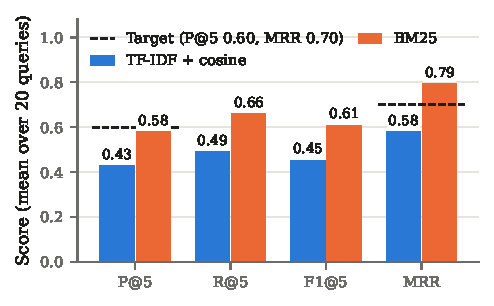
\includegraphics[width=\columnwidth]{figures/fig2_retrieval.pdf}
\caption{Retrieval quality of TF-IDF with cosine similarity and BM25. Dashed lines mark the targets fixed before evaluation.}
\label{fig:retrieval}
\end{figure}

\begin{figure}[t]
\centering
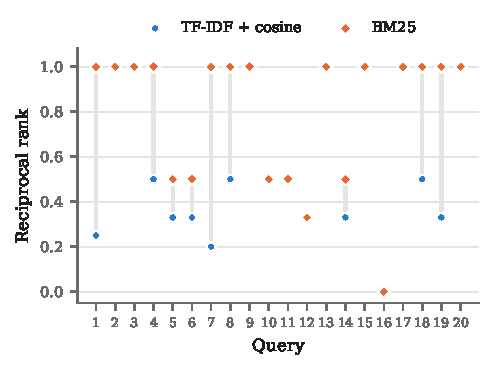
\includegraphics[width=\columnwidth]{figures/fig3_per_query_rr.pdf}
\caption{Reciprocal rank of the first relevant passage per question. Grey bars join the two rankers' results for the same question.}
\label{fig:perquery}
\end{figure}

\textbf{Ablation.} Every retrieval change was kept or rejected on this evaluation (Fig.~\ref{fig:ablation}, Table~\ref{tab:ablation}). Merging duplicates and lowering $b$ gave most of the gain; appending titles to passages and broadening the synonym dictionary made results worse. The heading fix lowered P@5 slightly because passages were re-cut, but it corrected wrong section names in citations from the 198-page fee policy, and citation correctness is a hard requirement. In the parameter sweep (Table~\ref{tab:sweep}), lowering $b$ helps because passage lengths vary widely, while $k_1$ matters little.

\begin{figure}[t]
\centering
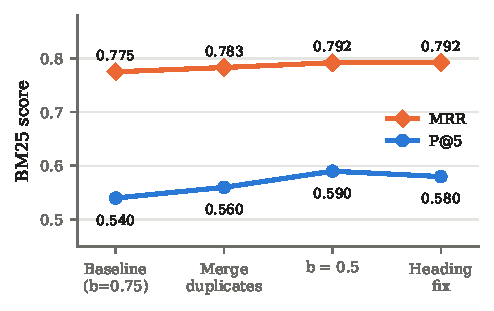
\includegraphics[width=\columnwidth]{figures/fig5_ablation.pdf}
\caption{BM25 P@5 and MRR after each accepted retrieval change.}
\label{fig:ablation}
\end{figure}

\begin{table}[t]
\caption{Retrieval Changes Tried (BM25)}
\label{tab:ablation}
\centering
\footnotesize
\setlength{\tabcolsep}{4pt}
\begin{tabular}{@{}L{3.0cm}cccl@{}}
\toprule
\textbf{Change} & \textbf{P@5} & \textbf{R@5} & \textbf{MRR} & \textbf{Kept} \\
\midrule
Baseline ($b=0.75$) & 0.540 & 0.626 & 0.775 & -- \\
Merge 226 duplicate passages & 0.560 & 0.644 & 0.783 & yes \\
$b=0.75\rightarrow0.5$ & 0.590 & 0.677 & 0.792 & yes \\
Heading fix (re-chunking) & 0.580 & 0.660 & 0.792 & yes \\
\midrule
Append title + section ($\times$1) & 0.540 & 0.622 & 0.797 & no \\
Append title + section ($\times$3) & 0.440 & 0.508 & 0.695 & no \\
Seven broader synonym groups & 0.560 & 0.644 & 0.783 & no \\
Drop passages under 8--12 words & \multicolumn{3}{c}{no gain at $b=0.5$} & no \\
\bottomrule
\end{tabular}
\end{table}

\begin{table}[t]
\caption{BM25 Parameter Sweep (After Merging Duplicates)}
\label{tab:sweep}
\centering
\footnotesize
\begin{tabular}{@{}ccccc@{}}
\toprule
$k_1$ & $b$ & \textbf{P@5} & \textbf{R@5} & \textbf{MRR} \\
\midrule
1.2 & 0.75 & 0.570 & 0.652 & 0.783 \\
1.5 & 0.75 & 0.560 & 0.644 & 0.783 \\
2.0 & 0.75 & 0.560 & 0.647 & 0.767 \\
1.5 & 0.90 & 0.570 & 0.655 & 0.704 \\
0.9 & 0.40 & 0.560 & 0.649 & 0.817 \\
1.2 & 0.50 & 0.590 & 0.677 & 0.792 \\
\textbf{1.5} & \textbf{0.50} & \textbf{0.590} & \textbf{0.677} & \textbf{0.792} \\
\bottomrule
\end{tabular}
\end{table}

\subsection{RQ2: Abstention}
Fig.~\ref{fig:gate} shows that the confidence score separates most, but not all, unanswerable questions. U02 (cricket) and U03 (essay) fall below $\tau=0.20$, while U04 (cafeteria menu, 0.23) and U05 (placement package, 0.22) score like the weakest answerable questions. U01 (pizza recipe) scores 0.70: \emph{recipe}, \emph{margherita} and \emph{pizza} are not in the index, so its only matched word is \emph{good}, which matches ``good academic standing'', and a single matched term makes the normalised score high. No threshold separates all 25 questions; the best accuracy of the gate alone is 88\%~\eqref{eq:tau}. The gate never refuses an answerable question (precision 1.00) and stops two off-topic questions before any LLM call; the model declines the other three, giving perfect abstention end to end with no false refusals (Table~\ref{tab:abstain}). This held in all six runs made with \code{gpt-oss-120b}.

\begin{figure}[t]
\centering
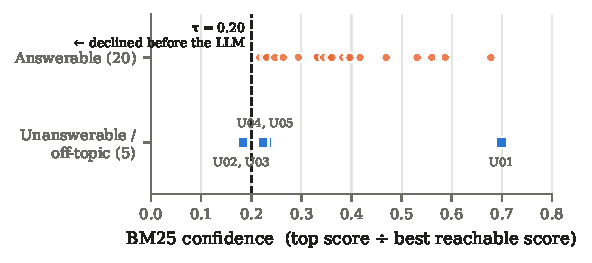
\includegraphics[width=\columnwidth]{figures/fig4_gate_confidence.pdf}
\caption{BM25 confidence~\eqref{eq:conf} of the 20 answerable and 5 unanswerable questions. Questions left of $\tau$ are declined without calling the LLM.}
\label{fig:gate}
\end{figure}

\begin{table}[t]
\caption{Abstention as Classification (Positive = Declined)}
\label{tab:abstain}
\centering
\footnotesize
\setlength{\tabcolsep}{2.2pt}
\begin{tabular}{@{}lcccccccc@{}}
\toprule
& \textbf{TP} & \textbf{FN} & \textbf{FP} & \textbf{TN} & \textbf{Acc.} & \textbf{Prec.} & \textbf{Rec.} & \textbf{F1} \\
\midrule
Gate only, BM25 & 2 & 3 & 0 & 20 & 0.88 & 1.00 & 0.40 & 0.57 \\
Gate only, TF-IDF & 1 & 4 & 0 & 20 & 0.84 & 1.00 & 0.20 & 0.33 \\
\textbf{Gate + prompt} & \textbf{5} & \textbf{0} & \textbf{0} & \textbf{20} & \textbf{1.00} & \textbf{1.00} & \textbf{1.00} & \textbf{1.00} \\
\bottomrule
\end{tabular}
\end{table}

\subsection{RQ3: Answer Quality and Groundedness}
Table~\ref{tab:versions} traces answer quality through the evaluation-driven changes; each row is a full run over the 25 questions. \emph{Neighbouring passages} cut wrong refusals from four to one: the model had correctly refused because the answer, for example the table of minimum class sizes, was in a passage next to the one retrieved. \emph{Prompt v3} removed the last wrong refusal by letting the model answer the covered part of a two-part question (``What is the anti-ragging policy and punishment for ragging?'') and state that the punishment is not specified. \emph{Prompt v4} was added after the v3 answer on disability support listed examples (``screen readers, ramps'') that do not appear in the source; v4 forbids such details, and the rerun removed them.

\begin{table}[t]
\caption{Answer Quality Across System Versions (\code{gpt-oss-120b})}
\label{tab:versions}
\centering
\footnotesize
\setlength{\tabcolsep}{3pt}
\begin{tabular}{@{}L{3.2cm}cccc@{}}
\toprule
\textbf{Version} & \textbf{Wrong ref.} & \textbf{Valid cit.} & \textbf{Correct} & \textbf{Complete} \\
\midrule
v1, top-5 passages only & 4/20 & 16/16 & -- & -- \\
v1 + neighbouring passages & 1/20 & 19/19 & 17/19 & 12/19 \\
v2: name the programme; keep all exceptions & 1/20 & 19/19 & 18/19 & 13/19 \\
v3: answer the covered part; heading fix & 0/20 & 20/20 & -- & -- \\
v3 + neighbours of all top-5 hits & 0/20 & 20/20 & -- & -- \\
\textbf{v4: add no unstated details} & \textbf{0/20} & \textbf{20/20} & \textbf{19/20} & \textbf{13/20} \\
\bottomrule
\multicolumn{5}{@{}L{8.2cm}@{}}{\scriptsize ``--'': run not graded in full. All runs declined 5/5 unanswerable questions and produced no invalid citation marker.}
\end{tabular}
\end{table}

The final system (Table~\ref{tab:final}) answered 19 of 20 questions correctly, with valid citations in every answer and no number that is absent from the passages. The 20 answers contain 90 statements: 68 with their own marker, 14 list items covered by the marker closing their list, 3 stating that the documents lack something, and 5 uncited. The 14 statements with no citation or word support below 0.6 were read against their passages; the other 76 passed the automatic check. Every cited statement is supported by its passage (citation precision 100\%), and 94\% of all statements are supported, above the 90\% target. All five failures are uncited sentences, mostly closing summaries such as ``So, you can use ChatGPT for early-stage idea generation~\dots'', which the strict rule counts as unsupported even when true; one of them is a wrong generalisation (Q08, Section~\ref{sec:discussion}).

\begin{table}[t]
\caption{Final Answer Quality (Prompt v4, 20 Answerable Questions)}
\label{tab:final}
\centering
\footnotesize
\begin{tabular}{@{}L{5.0cm}r@{}}
\toprule
\textbf{Measure} & \textbf{Result} \\
\midrule
\multicolumn{2}{@{}l}{\emph{Answer level}} \\
Factual correctness (accuracy) & 19/20 = 95\% \\
Evidence support & 20/20 = 100\% \\
Citation accuracy (document, page, paragraph) & 20/20 = 100\% \\
Completeness (conditions and exceptions kept) & 13/20 = 65\% \\
Answers with a number absent from all passages & 0/20 \\
\midrule
\multicolumn{2}{@{}l}{\emph{Statement level}} \\
Statements / covered by a citation & 90 / 83 (92\%) \\
Citation precision (cited statements supported) & \textbf{83/83 = 100\%} \\
Groundedness~\eqref{eq:ground} & \textbf{85/90 = 94\%} \\
\bottomrule
\end{tabular}
\end{table}

\subsection{Effect of the Language Model}\label{sec:model-effect}
Groq's free tier limits \code{gpt-oss-120b} to 200{,}000 tokens per day, and an evaluation run uses about 55{,}000. Once the limit was reached the system fell back to \code{gpt-oss-20b}, which answered most of two further runs. With the same retrieval and prompt, the smaller model gave valid citations in only 16/20 and 17/20 answers, against 20/20 for \code{gpt-oss-120b}, while abstention stayed at 5/5. The interface therefore states on every answer when a fallback model was used.

\subsection{RQ4: Spelling Correction}
For every answerable question, two adjacent letters in its longest word were swapped (e.g., \emph{attendance}$\rightarrow$\emph{attednance}). The speller restored all 20 words. With the typos, BM25 MRR fell from 0.792 to 0.629; after correction it returned to 0.792. The correction altered none of the 25 correctly spelled questions and made no change to the five off-topic ones, whose unknown words (\emph{pizza}, \emph{cricket}) have no near neighbour in the vocabulary.

\subsection{Efficiency}
Table~\ref{tab:eff} shows that every latency target is met by a wide margin on the reference laptop.

\begin{table}[t]
\caption{Efficiency on the Reference Machine}
\label{tab:eff}
\centering
\footnotesize
\begin{tabularx}{\columnwidth}{@{}Y L{3.0cm} l@{}}
\toprule
\textbf{Measure} & \textbf{Result} & \textbf{Target} \\
\midrule
Retrieval per question & median 0.2\,ms, max 0.8\,ms & $<500$\,ms \\
Spelling correction & 1--2\,ms & -- \\
Full answer (\code{gpt-oss-120b}) & median 0.9\,s, max 1.5\,s & $\approx5$\,s \\
Index load / full rebuild & 0.2\,s / 5.8\,s & -- \\
Index size on disk & 0.8\,MB & -- \\
\bottomrule
\end{tabularx}
\end{table}

\subsection{Comparison with Existing Research}
Table~\ref{tab:compare} compares our results with published work. The comparison with Liu et al.~\cite{liu2023verifiability} is the most direct, as both measure whether each generated sentence is supported by the source it cites. SNU Central's higher support rate comes from its design rather than a stronger model: the model may cite only passages that retrieval supplied, the application rejects any other citation, and the prompt forbids unstated details. The settings differ, however. Liu et al.\ evaluated commercial systems on open-web questions with independent annotators, whereas we evaluate 20 questions over a closed collection, graded by one author with AI assistance, with 76 of 90 statements passing an automatic check. Our result shows that the design \emph{can} reach high groundedness in a narrow domain; a larger, independently annotated test is needed to confirm it.

\begin{table*}[t]
\caption{Comparison with Published Results}
\label{tab:compare}
\centering
\footnotesize
\begin{tabularx}{\textwidth}{@{}L{3.4cm}YYY@{}}
\toprule
\textbf{Study} & \textbf{Setting} & \textbf{Reported result} & \textbf{SNU Central} \\
\midrule
Liu, Zhang and Liang~\cite{liu2023verifiability} & Four commercial generative search engines, open-web questions, human audit & 51.5\% of sentences fully supported by their citations; 74.5\% of citations support their sentence & 94\% of statements supported; 100\% of citations support their statement \\
Gao et al.\ (ALCE)~\cite{gao2023alce} & LLMs answering long-form questions with citations & Best models lack complete citation support for about half of their answers & 92\% of statements covered by a citation; every answer has a valid citation \\
Thakur et al.\ (BEIR)~\cite{thakur2021beir} & 18 retrieval datasets, zero-shot & BM25 a robust baseline on new domains; dense models often generalise poorly & BM25 beats TF-IDF by 36\% MRR on an unseen domain without training \\
Neupane et al.\ (BarkPlug v.2)~\cite{neupane2024barkplug} & RAG chatbot for one university's campus resources & Mean RAGAS score 0.96; user survey & Same goal; we report IR metrics and manually checked groundedness instead of an LLM-judged score \\
\bottomrule
\end{tabularx}
\end{table*}

\subsection{Discussion and Error Analysis}\label{sec:discussion}
\textbf{Retrieval is the bottleneck.} Five of the seven incomplete answers are retrieval misses rather than model errors: the ST212 penalty lists, the fourth-year 50\% attendance rule, the full disability-support policy (a one-paragraph handbook summary ranks higher), the grade-conversion tables, and the sentence stating that ragging is punishable. In each case the model said what the provided documents did not cover instead of guessing.

\textbf{The one factual error (Q08)} is a document-structure problem. The fee policy gives a refund schedule (75\%, 50\%, none) that applies to one certificate programme, but the programme has no heading in the PDF, so its passages fall under an unrelated section. The model labelled the rule as a postgraduate-certificate rule, as instructed, but still presented it as the default, while the general rule (refunds follow UGC norms and the admission notification) ranked fifth.

\textbf{Threats to validity.} The test set is small and was labelled by one person with AI assistance; relevance pools came from our own rankers, which can inflate recall; and $b$ and prompts v2--v4 were tuned on the questions they are evaluated on, so the final numbers are somewhat optimistic.

% ---------------------------------------------------------------------------------------------------
\section{Conclusions and Limitations}\label{sec:conclusion}

\subsection{Conclusions}
We presented SNU Central, a question-answering system that answers questions about university policies only from official documents and links every claim to its source. On 25 test questions over 39 documents, BM25 clearly outperformed TF-IDF (MRR 0.792 vs.\ 0.581) and was never worse on any question (RQ1). A length-normalised confidence gate plus a prompt-level refusal declined all five unanswerable questions with no false refusals (RQ2). Restricting the model to numbered passages and validating every citation produced answers in which 94\% of statements, and every cited statement, are supported, with 95\% of answers correct (RQ3). Spelling correction recovered the full retrieval loss caused by typos (RQ4). The system runs on an 8\,GB laptop at no cost, answers in under two seconds, and still shows cited passages when the LLM is unavailable. The most important design decision was to keep retrieval transparent and separately evaluated: every improvement and every failure could be traced to retrieval or to generation, and measured.

\subsection{Limitations}
(1)~The evaluation is small (25 questions, 92 judgments), labelled by one author with AI assistance, and $b$ and prompts v2--v4 were tuned on the same questions, so the numbers are somewhat optimistic. (2)~Completeness is the weakest result (13/20), mostly because lexical retrieval misses passages that share few words with the question. (3)~PDF tables are flattened and some programme headings are missing from the source, which caused the one factual error. (4)~Groundedness grading is partly automatic: 76 of 90 statements passed a word-support check rather than a full reading. (5)~Three of five off-topic questions are declined by the LLM rather than the gate, so abstention depends on the model. (6)~The free tier limits \code{gpt-oss-120b} to 200{,}000 tokens per day, and the fallback model cites less reliably. (7)~Coverage is limited to 39 text-based English PDFs from four public sources; five documents state no date. (8)~There is no conversation memory or personal eligibility assessment. (9)~The SNU Links policies may not be stored in a retrieval system without the university's permission, so the system is for local use by SNU students and cannot be deployed publicly as is.

\subsection{Future Work}
Promising next steps are hybrid retrieval that fuses BM25 with a dense retriever to reduce vocabulary mismatch; structure-aware ingestion that parses tables and recovers missing headings; a larger evaluation with student-written questions, several annotators and a held-out split; run-time entailment checks of each answer sentence against its cited passage; follow-up questions, document-discovery queries and category filters; detection of superseded policy versions; and an official deployment with the university's permission.

% ---------------------------------------------------------------------------------------------------
\begin{thebibliography}{13}
\footnotesize

\bibitem{ji2023hallucination}
Ji, Z., Lee, N., Frieske, R., Yu, T., Su, D., Xu, Y., Ishii, E., Bang, Y.J., Madotto, A. and Fung, P., 2023. Survey of hallucination in natural language generation. \textit{ACM Computing Surveys}, 55(12), pp.1--38.

\bibitem{lewis2020rag}
Lewis, P., Perez, E., Piktus, A., Petroni, F., Karpukhin, V., Goyal, N., K\"uttler, H., Lewis, M., Yih, W.T., Rockt\"aschel, T., Riedel, S. and Kiela, D., 2020, December. Retrieval-augmented generation for knowledge-intensive NLP tasks. In \textit{Advances in Neural Information Processing Systems 33 (NeurIPS 2020)} (pp.~9459--9474).

\bibitem{gao2023alce}
Gao, T., Yen, H., Yu, J. and Chen, D., 2023, December. Enabling large language models to generate text with citations. In \textit{Proceedings of the 2023 Conference on Empirical Methods in Natural Language Processing} (pp.~6465--6488).

\bibitem{salton1988term}
Salton, G. and Buckley, C., 1988. Term-weighting approaches in automatic text retrieval. \textit{Information Processing \& Management}, 24(5), pp.513--523.

\bibitem{robertson2009bm25}
Robertson, S. and Zaragoza, H., 2009. The probabilistic relevance framework: BM25 and beyond. \textit{Foundations and Trends in Information Retrieval}, 3(4), pp.333--389.

\bibitem{manning2008ir}
Manning, C.D., Raghavan, P. and Sch\"utze, H., 2008. \textit{Introduction to Information Retrieval}. Cambridge: Cambridge University Press.

\bibitem{damerau1964}
Damerau, F.J., 1964. A technique for computer detection and correction of spelling errors. \textit{Communications of the ACM}, 7(3), pp.171--176.

\bibitem{karpukhin2020dpr}
Karpukhin, V., Oguz, B., Min, S., Lewis, P., Wu, L., Edunov, S., Chen, D. and Yih, W.T., 2020, November. Dense passage retrieval for open-domain question answering. In \textit{Proceedings of the 2020 Conference on Empirical Methods in Natural Language Processing (EMNLP)} (pp.~6769--6781).

\bibitem{thakur2021beir}
Thakur, N., Reimers, N., R\"uckl\'e, A., Srivastava, A. and Gurevych, I., 2021, December. BEIR: A heterogeneous benchmark for zero-shot evaluation of information retrieval models. In \textit{Proceedings of the Neural Information Processing Systems Track on Datasets and Benchmarks (NeurIPS 2021)}.

\bibitem{rashkin2023ais}
Rashkin, H., Nikolaev, V., Lamm, M., Aroyo, L., Collins, M., Das, D., Petrov, S., Tomar, G.S., Turc, I. and Reitter, D., 2023. Measuring attribution in natural language generation models. \textit{Computational Linguistics}, 49(4), pp.777--840.

\bibitem{liu2023verifiability}
Liu, N.F., Zhang, T. and Liang, P., 2023, December. Evaluating verifiability in generative search engines. In \textit{Findings of the Association for Computational Linguistics: EMNLP 2023} (pp.~7001--7025).

\bibitem{es2024ragas}
Es, S., James, J., Espinosa-Anke, L. and Schockaert, S., 2024, March. RAGAs: Automated evaluation of retrieval augmented generation. In \textit{Proceedings of the 18th Conference of the European Chapter of the Association for Computational Linguistics: System Demonstrations} (pp.~150--158).

\bibitem{neupane2024barkplug}
Neupane, S., Hossain, E., Keith, J., Tripathi, H., Ghiasi, F., Golilarz, N.A., Amirlatifi, A., Mittal, S. and Rahimi, S., 2024. From questions to insightful answers: Building an informed chatbot for university resources. \textit{arXiv preprint arXiv:2405.08120}.

\end{thebibliography}

\end{document}
